%% ****** Start of file PhysRev_template.tex ****** %
%%
%%
%%   This template file is adapted from the sample provided in the REVTeX 4.2 distribution.
%%   Version 4.2a of REVTeX, January, 2015
%%
%%
%%   Copyright (c) 2015 The American Physical Society.
%%
%%   See the REVTeX 4 README file for restrictions and more information.
%%
%
% This is a template for producing manuscripts for use with REVTEX 4.2
% Copy this file to another name and then work on that file.
% That way, you always have this original template file to use.
%
% This template is set up for Phys. Rev. A.
% Replace pra with prb, prc, prd, or pre, respectively, to change to Phys. Rev. B, C, D, or E. 
\documentclass[aps,pra,twocolumn]{revtex4-2}
\usepackage{graphicx}

% Uncomment the line below if you intend to use ams symbols.
% You will need to download the appropriate ams packages from:
% http://www.ams.org/publications/authors/tex/tex

%\usepackage{amsmath}

\begin{document}

\title{Title of PHY480 report}
\author{Registration number}
\affiliation{Department of Physics \& Astronomy, University of Sheffield}

\date{\today}

\begin{abstract}
This \LaTeX\ document serves as a template for the PHY480 Semester~II report in \textit{Physical Review} format. The report should have a short abstract, up to about 200 words long, which summarizes the contents of the report, briefly describing its aims, methods, and main results.
It should be a single paragraph, and no references should appear in the abstract.
\end{abstract}

%\maketitle must follow title, authors, abstract, and keywords
\maketitle

% body of paper here - Use proper section commands
% References should be done using the \cite, \ref, and \label commands

\section{Introduction}
\label{sec:introduction}

The report should focus on the work done during semester two. The report should be written so as to be understandable to a non-specialist physics graduate and should follow the standard structure of a scientific paper. 

The report should be self-contained in the sense that it should not be necessary to have to re-read your report from semester~I in order to understand what the project is about. The report should therefore begin with a good introduction that explains the context of the work that you have done for your project. It should explain what your project was about, what you intended to do, and why this is important / useful / interesting. This introduction should include the references that underpin the work. There will, therefore, be some overlap with the literature review from semester I.

The report will be assessed independently by your supervisor and another academic. The second academic will normally be the same one who assessed your report in semester~I. This means that he/she will be someone who works in the same general area as the project topic (e.g. high-energy physics), but will {\em not} be familiar with the details of the project. Do not assume that the assessor should remember things from your Semester~I report. The marks of the second assessor carry equal weight as those of your supervisor, and so it is important that you explain clearly the context of your project and discuss any specialist techniques that you have used in language that is comprehensible to a physicist who is not working in exactly the same research area.



The main criteria for assessment will be the coherence of the scientific argument, the quality of the results obtained and their analysis, and the level of understanding displayed. However, marks may be deducted for poor written English, which  includes spelling (remember to use the `spell check' facility on the word processor), syntax and punctuation. Allowance will be made for students whose first language is not English. You will also lose marks for poor scientific style concerning equations, references, figures, tables, etc. 

The two assessors will award you a mark out of 50 for your report. The 50 marks are broken down into two categories:
\begin{description}
\item[Content] Aims and objectives, description of relevant theories / experimental techniques, quality of results obtained, interpretation and analysis of results.
 \textbf{(30 marks)}
\item[Clarity and presentation] Organisation and structure, conciseness, quality of language, clarity of presentation, references, quality and appropriateness of diagrams and figures.
 \textbf{(20 marks)}
\end{description}
The marks of the two assessors will be averaged, and will count as 50\% of the overall semester II mark. The other 50\% of the semester~II marks are awarded as follows:
\begin{description}
\item[25\%] Project attempt.
\item[25\%] Oral examination (a.k.a. the `\textit{viva}').
\end{description}
The overall semester~II mark counts as 75\% of the PHY480 module mark, with the other 25\% being your semester~I report. 

\textit{Special note for 2020.} The coronavirus pandemic makes the submission and assessment of lab-books impractical. You are therefore no longer required to submit your lab-book, and the 25 marks previously assigned for ``project attempt and lab-book'' will now be allocated entirely to the supervisor's project attempt mark.








\section{Preparation of the report}
The report should be written in appropriate scientific language. You should avoid the use of jargon, but if you do use jargon or acronyms, they should be defined before use.  

The project plan that you wrote for your semester I report should be attached verbatim as Appendix~\ref{App:project plan}. In the write up of your work in semester II, you should discuss how well you kept to the plan. If you departed significantly from the plan, you should explain why this was done.

\textit{Special guidance for 2020 reports}. This year, it is probable that many of you will have had to depart from your original plan due to the coronavirus pandemic. It is also possible that your project was affected by the industrial action. In these cases, please explain how your project was affected, and what revised plan you followed as a consequence. This statement should be included as Appendix~\ref{2020 special}. Please make a reference to this appendix when you discuss your project plan in the main body of your report. You can write as much as you like in the Appendix, as the appendices are not included in the word limit. 
If your project was not affected, please just write something like ``My project was not significantly affected either by the industrial action or the coronavirus'' in Appendix~\ref{2020 special}. Note that you might still have changed your plan even if there had been no industrial action or coronavirus. These changes to your plan should be discussed in your report, just as in all previous years.

 
The total length of the report should not exceed about 10,000 words, excluding the appendices. You can have as many words as you need for your appendices. A quick way to estimate the word count of a \LaTeX\ document is to create a PDF file, select and copy the relevant parts  of the report, and then paste into a word processor that has a word counting facility (e.g. WORD).

Some of you may wish to refer back to material from the preliminary work section of your first semester report. This is permitted, but you need to make sure that the semester II report is self-contained, as explained in Section~\ref{sec:introduction}. One option is to summarize the results from Semester~I in an Appendix called something like ``Summary of results from preliminary work in Semester~I'', and refer to this Appendix as needed within the main body of your report. If you include results from your Semester~I report, you \textit{must} make it clear that these results are from the previous report. For example, if you reproduce a data graph in the main body of your report, you must give a citation to your Semester~I report, such as \cite{semester 1 report}. The reports will be submitted through Turnitin, which will pick up the overlap with the previous report. Unless the origin of the material from the previous report is properly acknowledged, its re-use is considered plagiarism, as that material has already been assessed.

 The use of figures and tables can greatly improve the presentation of your project. For figures, the legends, annotations and axes labels, including units, must be clearly indicated. To include figures in a \LaTeX\ document, you first need to generate an image file (JPEG, PNG or PDF), and then use the {\tt includegraphics} command to include it in your document. Make sure that the axis labels are easily readable by ageing assessors with poor eyesight. Use the {\tt figure} environment and the {\tt caption} command to add a number and a caption to your figure. See the code for Figure \ref{fig:eclipse} for an example. There is no limit to the number of figures you can include. 
Figures taken or adapted from published sources should be appropriately referenced, as in Fig.~\ref{fig:eclipse}.

All equations should be numbered, as in eqn~\ref{E=mc2}:
\begin{equation}
\label{E=mc2}
E = mc^2 \, .
\end{equation}


% In two-column mode, this environment will change to single-column
% format so that long equations can be displayed. Use
% sparingly.
%\begin{widetext}
% put long equation here
%\end{widetext}

The report must be submitted according to strict Journal formatting rules. See Section~\ref{sec:format}.

\begin{figure}
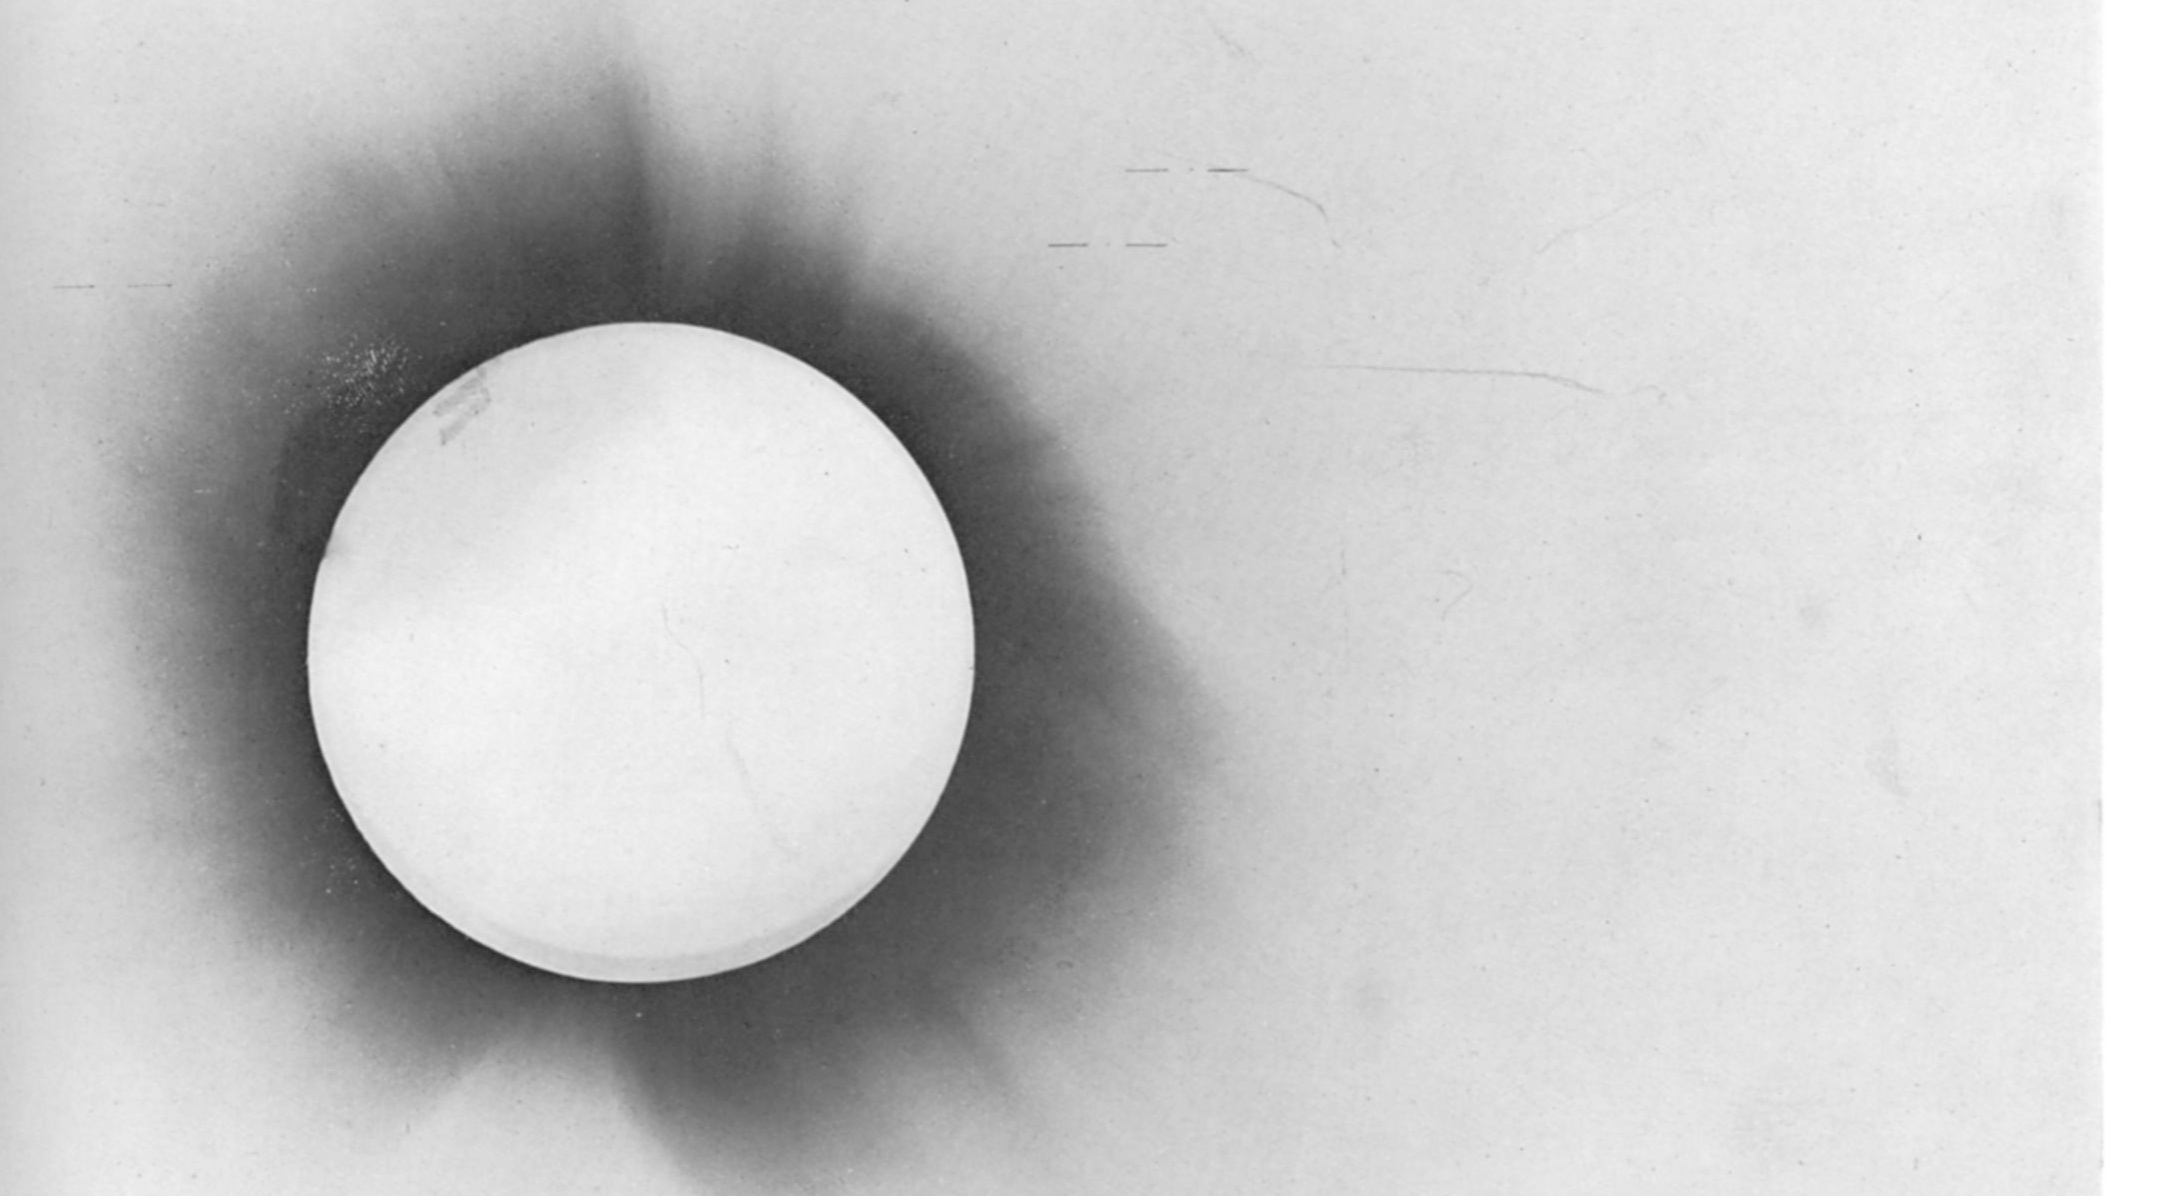
\includegraphics[width=\columnwidth]{Dyson.jpeg}
\caption{\label{fig:eclipse}Solar eclipse of 1919, which was studied to prove the bending of light by gravity. From \cite{Dyson}.}
\end{figure}

% figures should be put into the text as floats.
% Use the graphics or graphicx packages (distributed with LaTeX2e)
% and the \includegraphics macro defined in those packages.
% See the LaTeX Graphics Companion by Michel Goosens, Sebastian Rahtz,
% and Frank Mittelbach for instance.
%
% Here is an example of the general form of a figure:
% \begin{figure}
% \includegraphics{}%
% \caption{\label{}}
% \end{figure}
% Fill in the caption in the braces of the \caption{} command. Put the label
% that you will use with \ref{} command in the braces of the \label{} command.
% Use the figure* environment if the figure should span across the
% entire page. There is no need to do explicit centering.

% Surround figure environment with turnpage environment for landscape
% figure
% \begin{turnpage}
% \begin{figure}
% \includegraphics{}%
% \caption{\label{}}
% \end{figure}
% \end{turnpage}





\section{Structure of the report}

You are free to decide how best to present your work, but the following general structure should be used:

\begin{description}
\item[Front matter]	Title, registration number, date.

\item[Abstract]	The abstract should be up to about 200 words long and summarize the work and its conclusions. 

\item[Introduction]	The introduction should describe the project aims and give an overview of the background to the research topic, explaining what other people have done before you. 

\item[Main body] The main body of the report should begin with a discussion of any methods, theories, etc. relevant to the conduct of the project. You should then comment on your project plan. The results obtained and your analysis of them follows next. In some projects, it might be appropriate to summarize the key findings in a table. The final part is to discuss the results, putting them in their context and highlighting their significance. The structure will thus typically be as follows:
\begin{itemize}
\item methodology / experimental techniques;
\item discussion of any variations from your project plan submitted with your semester I report;
\item results, and their analysis;
\item critical discussion of results.
\end{itemize}

\item[Conclusion]	The report should end with a conclusion that summarizes the results obtained, places the work in its proper context and, if appropriate, makes suggestions for further related work. 

\item[References]	A reference list should be included for all works that are cited in the report. See Section~\ref{sec:refs}.

\item[Appendices]	Appendix A should be the project plan from your semester I report. Appendix B should be a statement about the effects of the industrial action and coronavirus on your project. Other appendices (e.g. computer source code, additional experimental results) should then be labelled consecutively with letters starting at \ref{other appendices}. 
\end{description}

% tables should appear as floats within the text
%
% Here is an example of the general form of a table:
% Fill in the caption in the braces of the \caption{} command. Put the label
% that you will use with \ref{} command in the braces of the \label{} command.
% Insert the column specifiers (l, r, c, d, etc.) in the empty braces of the
% \begin{tabular}{} command.
% The ruledtabular enviroment adds doubled rules to table and sets a
% reasonable default table settings.
% Use the table* environment to get a full-width table in two-column
% Add \usepackage{longtable} and the longtable (or longtable*}
% environment for nicely formatted long tables. Or use the the [H]
% placement option to break a long table (with less control than 
% in longtable).
% \begin{table}%[H] add [H] placement to break table across pages
% \caption{\label{}}
% \begin{ruledtabular}
% \begin{tabular}{}
% Lines of table here ending with \\
% \end{tabular}
% \end{ruledtabular}
% \end{table}

% Surround table environment with turnpage environment for landscape
% table
% \begin{turnpage}
% \begin{table}
% \caption{\label{}}
% \begin{ruledtabular}
% \begin{tabular}{}
% \end{tabular}
% \end{ruledtabular}
% \end{table}
% \end{turnpage} 

\section{Report format}
\label{sec:format}

The report should be submitted in one of two formats:
\begin{itemize}
\item Astrophysics projects should be submitted in the format of a paper in the \textit{Monthly Notices of the Royal Astronomical Society}.
\item All other reports should be submitted in the format of a paper in one of the \textit{Physical Review} Journals. You should choose the one that is most appropriate to your branch of physics:
\begin{itemize}
\item \textit{Physical Review A} for atomic, molecular, and optical physics, and quantum information;
\item \textit{Physical Review B} for condensed matter and materials physics;
\item \textit{Physical Review C} for nuclear physics;
\item \textit{Physical Review D} for particles, fields, gravitation, and cosmology;
\item \textit{Physical Review E} for statistical, nonlinear, biological, and soft matter physics.
\end{itemize}
\end{itemize}
If you are in any doubt about which of the \textit{Physical Review} formats to use, please ask your supervisor. The formats are, in fact, very similar, and you will not be penalized if you submit in the ``wrong''  \textit{Physical Review}  journal type.


The reports should be prepared following the instructions given on the journals' www sites.
\begin{itemize}
\item For \textit{Monthly Notices}, please see \url{https://academic.oup.com/mnras/pages/General_Instructions}.
\item For \textit{Physical Review} instructions, please see: \url{https://journals.aps.org/authors}.
\end{itemize}
The easiest way to get the right format is to use the \LaTeX\  files provided by the Journal.
\begin{itemize}
\item For \textit{Monthly Notices}, please see Section~2.1 of \url{https://academic.oup.com/mnras/pages/General_Instructions}. 
\item For \textit{Physical Review}, you  will need to use the REV\TeX~4.2 package. Information about how to get the REV\TeX~4.2 package is available at \url{http://journals.aps.org/revtex/}.
\end{itemize}
 If you do use these \LaTeX\ files, your report will automatically be set in the right format. Hence we strongly recommend using \LaTeX\ for your report.
 
 Some students may be unfamiliar with  \LaTeX\ and prefer to use a word-processor like WORD to prepare the report. This approach is acceptable, but the Journals only provide \LaTeX\ templates, and you will have to fiddle around to make your report have the right format. Download a recent paper from the appropriate journal, and reproduce it using your word processor. It is not necessary to reproduce the journal-specific headers and footers, and you will not be penalized if your report is not exactly in the right format, provided it looks like a good approximation to a pre-print paper in the relevant journal, as in this template. 








\section{References}
\label{sec:refs}


 You will need to cite the key papers that underpin your research in the introduction. You may need to give the references that explain the methodology that you are using, and you should  compare your own results to those that are published in the literature.

In giving the references, you should use standard scientific style, providing the following information: 
\begin{itemize}
\item author(s);
\item title of paper;
\item journal name, volume number, pages (or article ID number), year.
\end{itemize}
See \cite{Dyson} or  \cite{Einstein} for examples. If you cite books \cite{good book} or longer review articles, you should give the specific section of the book to which you are referring. 

The references should be numbered for \textit{Physical Review} style (as in this report template), or follow the Harvard (name, date) system for  \textit{Monthly Notices} format. LaTeX users might find it helpful to use BibTeX \cite{BibteX}, while WORD users might want to consider using EndNote \cite{Endnote}.
If you are uncertain about any aspects of referencing, please look up the on-line tutorials provided by the library and refer to the Departmental referencing style for Physics \& Astronomy \cite{Referencing}. 


\section{Submitting the report}

% Hard copy submissions are not possible in 2020
% The following text is kept for use next year.
%You should submit \textbf{three} printed copies of your report together with your lab-book by Friday of week 12 of the Second Semester. Your printed reports should be mounted in the plastic binders that can be collected from F10.  
%The electronic version of your report should be submitted at the same time as the printed copies.%

You should submit your report electronically using the Turnitin anti-plagiarism portal of PHY480 by \textbf{Friday of week 12 of Semester~II} (29th May). Please name your file: ``XXXXXXXXX-PHY480-report'', where ``XXXXXXXXX'' is your registration number. You should make sure that you comply stringently with the University's plagiarism guidelines \cite{plagiarism}. Note that minor changes to the original wording do not constitute a defence against accusations of plagiarism. If you are uncertain about any aspects of  plagiarism, please look up the on-line tutorials provided by the library \cite{Referencing}. 

% References
%
% LaTeX experts may wish to use BibTeX.
% If you do use BibTeX, please follow the guidance below.
% If you do not have time to learn how to use BibTeX, you can do the references just by using the following code, as in this template:  
% \begin{thebibliography}{99}
% \bibitem{Bloggs} J. Boggs ...
% \end{thebibliography}
%
% For BibTeX users:
% Uncomment the line below.
%\bibliography{basename of .bib file}
% You should use BibTeX and apsrev.bst for references
% Choosing a journal automatically selects the correct APS
% BibTeX style file (bst file), so only uncomment the line
% below if necessary.
%\bibliographystyle{apsrev4-2}% 
%



\begin{thebibliography}{99}
% The 99 argument allows you to have up to 99 references. If you have more than 99 (not recommended!), you will need to change it to 999.

\bibitem{semester 1 report}
Student \textit{registration number}, PHY480 Semester~1 Report, University of Sheffield, 2019.

\bibitem{Dyson}
F.W. Dyson, A.S. Eddington, and C.R. Davidson, ``Determination of the Deflection of Light by the Sun's Gravitational Field, from Observations Made at the Solar eclipse of May 29, 1919'', Phil. Trans. Roy. Soc. A. \textbf{220}, 291--333 (1920).

\bibitem{Einstein}
A. Einstein, ``Zur Elektrodynamik bewegter K\"{o}rper'', Annalen der Physik, \textbf{17}, 891--921 (1905).


\bibitem{good book}
M. Fox, \textit{Optical properties of solids}, 2nd edn (Oxford University Press, 2010), pp 167 -- 174.


\bibitem{BibteX}
See http://www.bibtex.org/ 

\bibitem{Endnote}
See https://www.sheffield.ac.uk/cics/endnote

\bibitem{Referencing}
See https://www.sheffield.ac.uk/library/idlt/referencing

\bibitem{plagiarism}
See https://www.sheffield.ac.uk/ssid/exams/plagiarism




\end{thebibliography}


% The following sections are appendices. 

\appendix

\section{Semester One Project Plan}
\label{App:project plan}
Appendix A  should be identical to the project plan from your semester~I report. 

\section{Effect of industrial action and coronavirus}
\label{2020 special}
Please give a statement in this appendix of the effect of the industrial action and coronavirus on your project. There is no word limit. If there was no significant effect, just write something like ``The industrial action and coronavirus had no significant effect on my project.''


\section{Other stuff}
\label{other appendices}
You can have as many other appendices as you need. These appendices could contain, for example, computer source code, additional experimental results, lengthy tables of data, etc.  They could also contain material from your Semester~I report to which you wish to make reference. These appendices should be labelled consecutively with letters, starting at \ref{other appendices}.


\end{document}









